\documentclass[a4paper]{article}

\usepackage[english]{babel}
\usepackage[utf8]{inputenc}
\usepackage{amsmath}
\usepackage{graphicx}
\usepackage{color}
\usepackage{float}
\usepackage{listings}
\definecolor{keywords}{RGB}{255,0,90}
\definecolor{comments}{RGB}{0,0,113}
\definecolor{red}{RGB}{160,0,0}
\definecolor{green}{RGB}{0,150,0}
\definecolor{codegreen}{rgb}{0,0.6,0}
\definecolor{codegray}{rgb}{0.5,0.5,0.5}
\definecolor{codepurple}{rgb}{0.58,0,0.82}
\definecolor{backcolour}{rgb}{0.95,0.95,0.92}
\definecolor{brown}{rgb}{0.59, 0.29, 0.0}
\definecolor{beaublue}{rgb}{0.74, 0.83, 0.9}
\definecolor{orange}{rgb}{1.0, 0.5, 0.0}
\definecolor{darkslategray}{rgb}{0.18, 0.31, 0.31}
\definecolor{deepblue}{rgb}{0,0,0.5}
\definecolor{deepred}{rgb}{0.6,0,0}
\definecolor{deepgreen}{rgb}{0,0.5,0}
\definecolor{auburn}{rgb}{0.43, 0.21, 0.1}
\definecolor{bistre}{rgb}{0.24, 0.17, 0.12}
\definecolor{babyblue}{rgb}{0.54, 0.81, 0.94}
\definecolor{ballblue}{rgb}{0.13, 0.67, 0.8}
\lstdefinestyle{myMatlabstyle}{
	language=Matlab,
	backgroundcolor=\color{white},   
	commentstyle=\color{deepgreen},
	keywordstyle=\color{black},
	identifierstyle=\color{black},
	numberstyle=\tiny\color{codegray},
	stringstyle=\color{purple},
	basicstyle=\footnotesize,
	breakatwhitespace=false,         
	breaklines=true,                 
	captionpos=b,                    
	keepspaces=true,                 
	numbers=left,                    
	numbersep=5pt,                  
	showspaces=false,                
	showstringspaces=false,
	showtabs=false,                  
	tabsize=2
}
\lstdefinestyle{myPythonstyle}{
	language=Python, 
	basicstyle=\ttfamily\small, 
	keywordstyle=\color{blue},
	commentstyle=\color{green},
	stringstyle=\color{red},
	showstringspaces=false,
	identifierstyle=\color{black},
}
\lstset{language=Matlab,frame=single}
\lstset{language=Python,frame=single}
\usepackage[colorinlistoftodos]{todonotes}
\usepackage[scale=0.75]{geometry}
	\title{Estimating speech from lip movement}

\author{Jithin D. George, Ronan Keane, Connor Zellmer}

\date{\today}

\begin{document}
\maketitle

\begin{abstract}

\end{abstract}

\section{Introduction and Overview}
\label{sec:introduction}

\begin{figure}[H] 
	\centering
	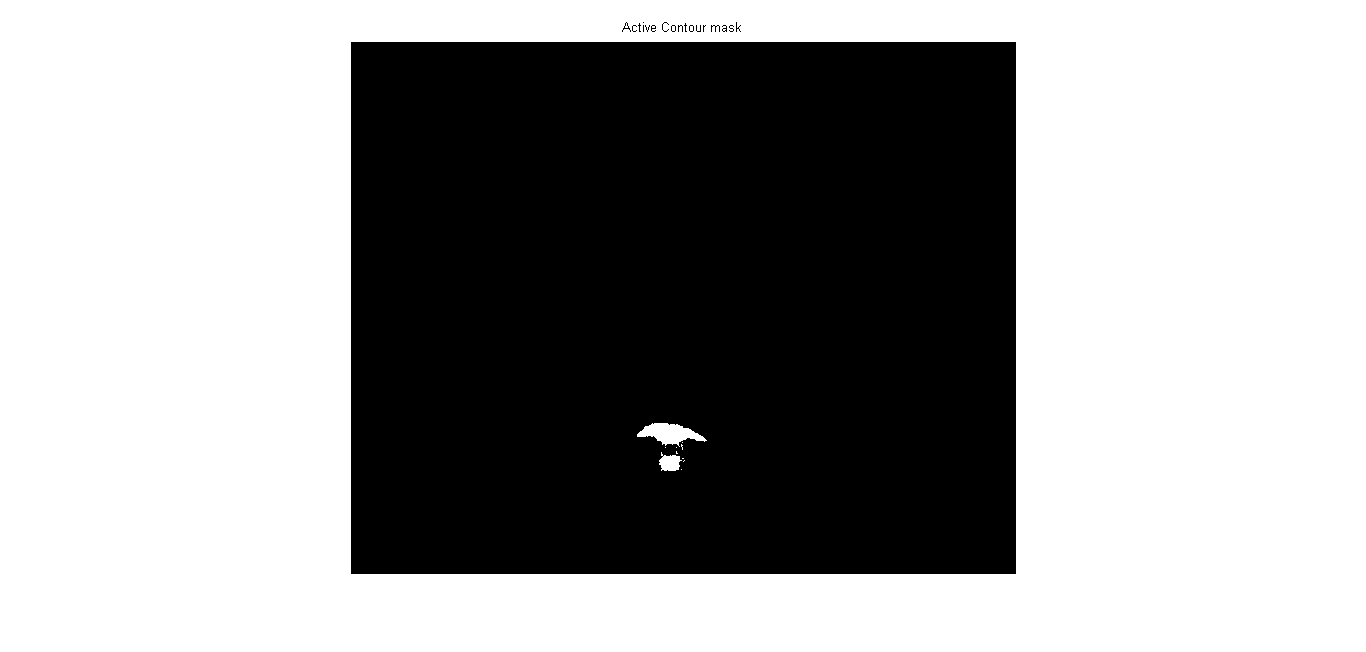
\includegraphics[width=0.7\textwidth]{active}
	\caption{Active Contour}	
\end{figure}

\begin{figure}[H] 
	\centering
	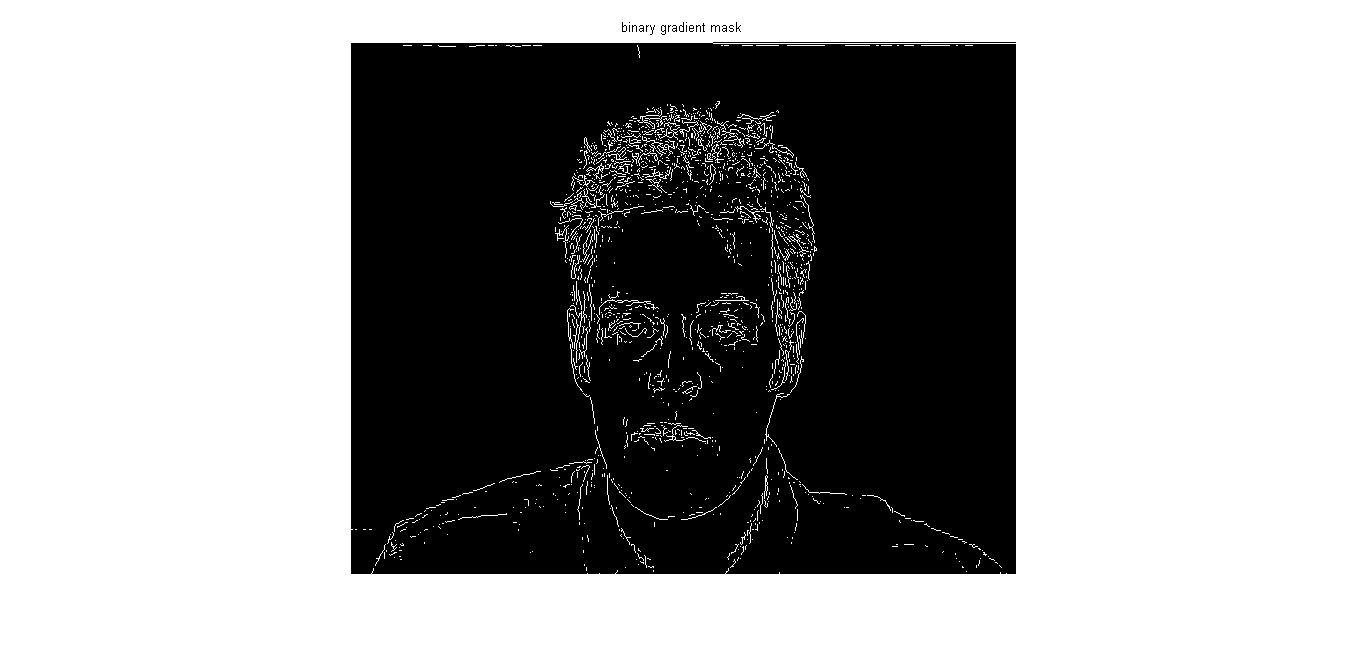
\includegraphics[width=0.7\textwidth]{binary}
	\caption{Binary Gradient}	
\end{figure}
\section{Theoretical Background}
\label{sec:theory}


\section{Implementation and Development}




\section{Computational Results}

\section{Summary and Conclusions}



\begin{thebibliography}{1}
	\bibitem{key-1}J. Proctor, S. Brunton and J. N. Kutz, Dynamic mode decomposition with control, arXiv:1409.6358.
	
	\bibitem{key-2}J. Grosek and J. N. Kutz, Dynamic mode decomposition for real-time background/foreground separation in video, arXiv:1404.7592.
	
	

\end{thebibliography}

\newpage

\appendix
%dummy comment inserted by tex2lyx to ensure that this paragraph is not empty


\section{MATLAB Functions used}
\begin{itemize}
\item \textbf{[U,S,V]=svd(A): } \\ This function performs the singular value decomposition of A and returns U,S and V.
\item \textbf{mat2gray(A): } \\ This function converts a matrix to greyscale.

\end{itemize}

\section{MATLAB Code}

\subsection{hw4.m}
\begin{lstlisting}[style=myMatlabstyle]
obj=VideoReader('vid1.mpg');
vidFrames = read(obj);
numFrames = get(obj,'numberOfFrames');
[mov]= getmovout(vidFrames,numFrames-1);
X=frame2im(mov(50));
A=rgb2gray(X);
mask = zeros(size(A));
mask(400:450,320:400) = 1;
bw = activecontour(A,mask,300);
figure, imshow(bw), title('Active Contour mask');
[~, threshold] = edge(A, 'sobel');
fudgeFactor = .5;
BWs = edge(A,'sobel', threshold * fudgeFactor);
figure, imshow(BWs), title('binary gradient mask');
\end{lstlisting}

\end{document}